%% This is file `elsarticle-template-1-num.tex',
%%
%% Copyright 2009 Elsevier Ltd
%%
%% This file is part of the 'Elsarticle Bundle'.
%% ---------------------------------------------
%%
%% It may be distributed under the conditions of the LaTeX Project Public
%% License, either version 1.2 of this license or (at your option) any
%% later version.  The latest version of this license is in
%%    http://www.latex-project.org/lppl.txt
%% and version 1.2 or later is part of all distributions of LaTeX
%% version 1999/12/01 or later.
%%
%% Template article for Elsevier's document class `elsarticle'
%% with numbered style bibliographic references
%%
%% $Id: elsarticle-template-1-num.tex 149 2009-10-08 05:01:15Z rishi $
%% $URL: http://lenova.river-valley.com/svn/elsbst/trunk/elsarticle-template-1-num.tex $
%%
\documentclass[preprint,11pt]{elsarticle}

%% Use the option review to obtain double line spacing
%% \documentclass[preprint,review,12pt]{elsarticle}

%% Use the options 1p,twocolumn; 3p; 3p,twocolumn; 5p; or 5p,twocolumn
%% for a journal layout:
%% \documentclass[final,1p,times]{elsarticle}
%% \documentclass[final,1p,times,twocolumn]{elsarticle}
%% \documentclass[final,3p,times]{elsarticle}
%% \documentclass[final,3p,times,twocolumn]{elsarticle}
%% \documentclass[final,5p,times]{elsarticle}
%% \documentclass[final,5p,times,twocolumn]{elsarticle}

%% The graphicx package provides the includegraphics command.
\usepackage{graphicx}
%% The amssymb package provides various useful mathematical symbols
\usepackage{amssymb}
\usepackage{subcaption}
\usepackage{float}
\usepackage{booktabs}
\usepackage{url}
%% The amsthm package provides extended theorem environments
%% \usepackage{amsthm}

%% The lineno packages adds line numbers. Start line numbering with
%% \begin{linenumbers}, end it with \end{linenumbers}. Or switch it on
%% for the whole article with \linenumbers after \end{frontmatter}.
\usepackage{lineno}
\usepackage{newtxtext,newtxmath,amsmath,fixme}

%%%%%%
\usepackage{tikz}
\usetikzlibrary{shapes.geometric, arrows.meta, positioning}

\tikzstyle{startstop} = [rectangle, rounded corners, minimum width=2.5cm, minimum height=1cm,text centered, draw=black, fill=gray!20]
\tikzstyle{process} = [rectangle, minimum width=2.5cm, minimum height=1cm, text centered, draw=black, fill=blue!10]
\tikzstyle{decision} = [diamond, minimum width=3cm, minimum height=1cm, text centered, draw=black, fill=yellow!20]
\tikzstyle{arrow} = [thick,->,>=stealth]
\usepackage{float}
%%%%%%%%%%%%%%%%%%%%



%% natbib.sty is loaded by default. However, natbib options can be
%% provided with \biboptions{...} command. Following options are
%% valid:

%%   round  -  round parentheses are used (default)
%%   square -  square brackets are used   [option]
%%   curly  -  curly braces are used      {option}
%%   angle  -  angle brackets are used    <option>
%%   semicolon  -  multiple citations separated by semi-colon
%%   colon  - same as semicolon, an earlier confusion
%%   comma  -  separated by comma
%%   numbers-  selects numerical citations
%%   super  -  numerical citations as superscripts
%%   sort   -  sorts multiple citations according to order in ref. list
%%   sort&compress   -  like sort, but also compresses numerical citations
%%   compress - compresses without sorting
%%
%% \biboptions{comma,round}

% \biboptions{}

\journal{Nuclear Instruments and Methods A}

\begin{document}

\begin{frontmatter}

%% Title, authors and addresses

%\title{Millikelvin precise temperature monitoring system for the ProtoDUNE-SP LArTPC detector at CERN}

\title{R\&D on milikelvin-precision temperature sensing with FBG fibers for cryogenic environments}

%% use the tnoteref command within \title for footnotes;
%% use the tnotetext command for the associated footnote;
%% use the fnref command within \author or \address for footnotes;
%% use the fntext command for the associated footnote;
%% use the corref command within \author for corresponding author footnotes;
%% use the cortext command for the associated footnote;
%% use the ead command for the email address,
%% and the form \ead[url] for the home page:
%%
%% \title{Title\tnoteref{label1}}
%% \tnotetext[label1]{}
%% \author{Name\corref{cor1}\fnref{label2}}
%% \ead{email address}
%% \ead[url]{home page}
%% \fntext[label2]{}
%% \cortext[cor1]{}
%% \address{Address\fnref{label3}}
%% \fntext[label3]{}


%% use optional labels to link authors explicitly to addresses:
%% \author[label1,label2]{<author name>}
%% \address[label1]{<address>}
%% \address[label2]{<address>}


%\author[ific]{J. \'Alvarez, H. Amar, C. Ben\'itez, J. Cap\'o, A. Cervera, J. Mart\'in-Albo, L. Molina, M. Sorel, J. Soto,  M. Tuzi, J. Ure\~na, N. Yahlali  }

% More authors to be added
\author{ 
V. García, J. Álvarez, S. Benítez, J. Capó, A. Cervera, J. Soto, S. Teruel, N. Yahlali}

\affiliation{
    organization={Instituto de Física Corpuscular (IFIC), CSIC--Universitat de València},
    city={Valencia},
    country={Spain}
}


% \address[ific]{Instituto de F\'isica Corpuscular, CSIC \& University of Valencia, Spain}



\date{\today}

\begin{abstract}

Precise temperature monitoring, at the level of a few millikelvin, is essential for the operation of large-scale cryostats equipped with recirculation systems. In particular, the performance of Liquid Argon Time Projection Chambers (LArTPCs), such as those planned for the DUNE experiment, strongly depends on efficient argon purification and mixing, which can be characterized through a sufficiently dense grid of high-precision temperature sensors.
In environments where the use of conventional electrical sensors, such as Resistance Temperature Detectors (RTDs), may be limited by the presence of high electric fields, Fiber Bragg Grating (FBG) sensors provide an attractive alternative. FBGs offer electrical insulation, immunity to electromagnetic interference, and the possibility of multiplexing multiple sensors along a single optical fiber, making them particularly suitable for large cryogenic systems.
In this article, we present the principles and experimental validation of a temperature monitoring system based on an array of FBG sensors, with particular emphasis on the techniques required to achieve millikelvin-level temperature precision. The results demonstrate the potential of FBG arrays for high-precision temperature monitoring in large-scale cryogenic systems.

    % Outline of the abstract
%    \begin{itemize}
%    \item Brief context on Fiber Bragg Gratings (FBGs) for temperature measurement.
% \ Objective: Evaluate the thermal sensitivity and repeatability of differently coated fibers.
%        \item Method: Cryogenic pressure-based setup using liquid nitrogen.
%        \item Key findings to be added... \\
%    \end{itemize}

%    The Deep Underground Neutrino Experiment (DUNE) requires extreme thermal stability within its Liquid Argon (LAr) cryostats... Specifically, temperature gradients must be maintained below 20 mK to stabilize the electron drift velocity in the LArTPC. In this work, we present a thermal sensitivity repeatability study of Fiber Bragg Grating (FBG) sensors conducted in a cryogenic pressure-based nitrogen setup. Our results demonstrate the reliability of different coated FBG sensors...


\end{abstract}

\begin{keyword}
Detectors \sep Liquid nitrogen \sep FBG \sep cryogenics \sep RTD \sep Temperature
%% keywords here, in the form: keyword \sep keyword

%% MSC codes here, in the form: \MSC code \sep code
%% or \MSC[2008] code \sep code (2000 is the default)

\end{keyword}

\end{frontmatter}

\tableofcontents


\linenumbers

% ==========================================
\section{Introduction}
% ==========================================
\label{sec:intro}

Fiber Bragg Gratings (FBGs) constitute an emerging technology that has been extensively studied and widely used for structural health monitoring in industrial and civil engineering applications at ambient temperatures. However, comparatively limited research has been performed on their use in cryogenic environments. 
The development of FBG-based sensing systems for cryogenic applications is being pursued in the context of the Deep Underground Neutrino Experiment (DUNE), where precise temperature measurements in its large liquid-argon detectors are essential for understanding and optimizing the cryogenic recirculation system.

DUNE employs Liquid Argon Time Projection Chamber (LArTPC) technology to produce a three-dimensional image of the trajectories of charged particles. Liquid-argon mixing is promoted by injecting relatively warm liquid argon through the bottom of the detector at well-defined locations, referred to as inlets, while a set of pumps provides continuous recirculation \cite{abi2020deepundergroundneutrinoexperiment, dunecollaboration2023dunefardetectorvertical}. Computational Fluid Dynamics (CFD) simulations have been used to optimize the number and location of the inlets and recirculation pumps, as well as the temperature of the incoming liquid argon relative to the bulk. These simulations predict a stationary vertical temperature gradient of approximately 20 mK. Such gradients have also been observed in the DUNE prototypes at CERN, which are approximately half the height of the final detectors. Measuring these gradients with a precision better than 5 mK is therefore crucial for validating the CFD models and understanding the performance of the liquid-argon recirculation system.
%Natural convection then contributes to the establishment of a recirculation pattern that progressively distributes the purified argon throughout the detector volume, resulting in electron lifetimes exceeding 20 ms. 

%Ionization electrons produced by particle interactions drift through the liquid argon towards the anode planes, where they are detected and read out. Efficient liquid-argon recirculation and purification are essential to reduce electronegative impurities to the parts-per-billion level, since these impurities absorb drifting electrons and consequently degrade the quality of the reconstructed images. 

%An FBG consists of a periodic modulation of the refractive index of an optical fiber, which causes light at a specific wavelength—the Bragg wavelength—to be reflected. An interrogator sends broadband or wavelength-tunable light through the fiber and analyzes the reflected signal. The Bragg wavelength depends on both the temperature and the strain at the location of the FBG. Consequently, changes in the reflected wavelength provide information about the local temperature and strain. If the strain is sufficiently well controlled or independently characterized, the temperature can be inferred from the wavelength shift.

%FBG technology is complementary to conventional Resistance Temperature Detectors (RTDs), and the choice between the two depends on the specific application. While RTDs require electrical cables for signal readout, which are generally robust and relatively easy to handle, optical fibers are typically more delicate and require greater care during installation. FBGs nevertheless offer a major advantage in applications requiring a large number of sensors: tens of FBG sensors can be multiplexed along a single optical fiber, whereas conventional RTDs typically require four electrical wires per sensor. RTDs are intrinsically insensitive to strain, which can simplify the determination of temperature and potentially enable higher measurement accuracy. FBGs, on the other hand, are dielectric and therefore particularly well suited to environments with high electric fields.



%The Phase-I DUNE detector consists of two modules: one based on the Vertical Drift (FD-VD) concept and the other on the Horizontal Drift (FD-HD) concept. The FD-VD module has two anode planes located at the top and bottom of the cryostat, with a cathode positioned at mid-height. The FD-HD module consists of four independent drift volumes, each delimited by a sandwich of three anode planes and two cathode planes.

%RTD technology will be used in the FD-HD detector. Twenty-five arrays of eight sensors each will instrument each anode plane, providing a detailed temperature map with particular emphasis on the vertical temperature gradient. A similar configuration is not feasible in the FD-VD detector because the cathode is maintained at a potential of approximately 320 kV. Electrical cables cannot therefore be deployed in the vicinity of the active volume, as they would have to cross regions at significantly different electric potentials.

%The current design for the DUNE Far Detector - Vertical Drift (FD-VD) module therefore foresees the deployment of several optical fibers vertically across the detector active volume. Each fiber will contain an array of approximately 20–30 FBG sensors, enabling measurements of the vertical temperature gradient at multiple locations throughout the detector.
In the current design for the DUNE Far Detector - Vertical Drift (FD-VD) module, several optical fibers will be installed vertically across the detector active volume. This approach avoids the need for electrical cables in the vicinity of the active volume, where the cathode operates at a high voltage of approximately 320 kV. Each fiber will contain an array of approximately 20–30 FBG sensors, enabling temperature measurements at multiple locations along the vertical direction and providing a detailed characterization of the temperature gradient.

The requirement to measure temperature with a precision better than 5 mK translates into stringent requirements on both the interrogator and the FBG fibers. In particular, the temperature sensitivity of an FBG depends significantly on the properties of its fiber coating, especially at cryogenic temperatures. Several coating technologies suitable for operation in cryogenic environments will therefore be investigated as part of this R\&D program.


%\subsection{RTD sensors (PT-103)}
%Definir las características 

% ==========================================
%\section{State of the art of FBG base temperature sensing (Jordi+Sara)} 
%\section{Influence of coating in FBG sensitivity} (commented by Nadia, see below)
\section{Cryogenic sensing with FBGs}
% ==========================================
\label{sec:fbgs}


---------------------------------------------------------------------------------------------------------------------------------------------------------------------------------------------------------------------------------------------------------------------------------------------------------------------------------------------------------------------------------------------
%\subsection{Sensitivity contributions} (commented by Nadia, see below)
\subsection{Sensitivity influencing factors}
\label{subsec:sensitivity}

%------------------------------------------------------
% \begin{itemize}
%     \item Overview of optical fibers as sensors.
%     \item Principles of Fiber Bragg Gratings (FBGs).
%     \item The Bragg condition formula:
%     \begin{equation}
%         \lambda_B = 2 n_{\text{eff}} \Lambda
%     \end{equation}
%     where $\lambda_B$ is the Bragg wavelength, $n_{\text{eff}}$ is the effective refractive index, and $\Lambda$ is the grating period \cite{Othonos1997}.
%     \item Explanation of how temperature and strain affect the Bragg wavelength:
%     \begin{equation}
%         \frac{\Delta \lambda_B}{\lambda_B} = (1 - P_e)\varepsilon + (\alpha + \xi)\Delta T
%     \end{equation}
%     where $P_e$ is the photo-elastic coefficient, $\varepsilon$ is strain, $\alpha$ is the thermal expansion coefficient, and $\xi$ is the thermo-optic coefficient \cite{Rao1997}.
% \end{itemize}

\begin{itemize}
    \item Current advancements in FBG thermal sensitivity at cryogenic temperatures \cite{James2002}.
    \item Comparison of standard setups used in the literature (e.g., climatic chambers, helium cryostats) \cite{Lupi2008}.
    \item Why our specific pressure-based approach provides novel insights or specific validation?
\end{itemize}

At ambient temperature ($300~\text{K}$), the wavelength shift of a bare silica FBG is governed almost entirely by the thermo-optic effect of fused silica ($dn/dT \approx 8.6 \times 10^{-6}~\text{K}^{-1}$), which accounts for over 90\% of the standard $\sim$10~pm/K sensitivity, while thermal expansion contributes negligibly ($\alpha_{\text{silica}} \approx 0.5 \times 10^{-6}~\text{K}^{-1}$). In cryogenic conditions ($77$--$93~\text{K}$), however, the thermo-optic coefficient drops by nearly an order of magnitude (down to $<1.0 \times 10^{-6}~\text{K}^{-1}$) and the thermal expansion of silica becomes negligible ($\alpha_{\text{silica}} < 0.2 \times 10^{-6}~\text{K}^{-1}$), causing the intrinsic sensitivity of bare silica gratings to collapse to less than $1.5~\text{pm/K}$~\cite{Lupi2008,Salin2008,Rajan2013}. To recover high thermal responsivity in cryogenic noble liquid detectors, the optical fiber is functionalized with a polymeric coating that serves as a mechanical thermal transducer:
\begin{equation}
    \frac{\Delta \lambda_B}{\lambda_B} = (\alpha_{\text{silica}} + \zeta) \Delta T + (1 - p_e) \epsilon_z,
    \label{eq:fbg_coating_strain}
\end{equation}
where $\zeta = (1/n)(dn/dT)$ is the normalized thermo-optic coefficient, $p_e \approx 0.22$ is the effective photoelastic constant, and $\epsilon_z$ is the total longitudinal strain in the silica core. Under tension-free mounting 
%in the calibration capsule (where external mechanical loads are negligible, $\epsilon_z^{\text{mech}} \approx 0$), 
the axial strain is purely thermally driven by the differential contraction between the polymer jacket and the glass: $\epsilon_z = \eta (\alpha_{\text{coating}} - \alpha_{\text{silica}}) \Delta T$, where $\eta \le 1$ represents the interfacial strain-transfer efficiency. Because polymer materials maintain cryogenic thermal expansion coefficients orders of magnitude higher than silica ($\alpha_{\text{coating}} \sim 15$--$35 \times 10^{-6}~\text{K}^{-1}$ at $77~\text{K}$, as summarized in Table~\ref{tab:material_cte}), the contracting jacket exerts a strong axial compressive strain on the fiber core, enhancing the cryogenic thermal sensitivity up to $15$--$35~\text{pm/K}$~\cite{Lupi2008,Zhao2007,Rajan2013}.

\begin{table}[htpb]
    \centering
    \footnotesize
    \setlength{\tabcolsep}{4.5pt}
    \caption{Thermal expansion properties and integrated cryogenic contraction of the optical fiber constituents.}
    \label{tab:material_cte}
    \begin{tabular}{lcccc}
        \toprule
        \textbf{Material} & $\boldsymbol{\alpha_{300\,\text{K}}}$ & $\boldsymbol{\alpha_{77\,\text{K}}}$ & $\boldsymbol{\Delta L/L}$ & \textbf{Structural Role} \\
                          & ($10^{-6}\,\text{K}^{-1}$)           & ($10^{-6}\,\text{K}^{-1}$)          & ($300\to 77\,\text{K}$)   &                          \\
        \midrule
        Fused silica        & $\sim 0.5$    & $< 0.2$   & $\sim 0.01\%$       & Core / Cladding glass~\cite{NIST_CryoMaterials} \\
        Polyimide           & $30$--$40$    & $12$--$20$ & $\sim 0.4$--$0.6\%$ & Primary buffer coating~\cite{Zhao2007,NIST_CryoMaterials} \\
        PEEK                & $45$--$50$    & $20$--$30$ & $\sim 1.0$--$1.2\%$ & Thermoplastic jacket~\cite{NIST_CryoMaterials} \\
        Ormocer / Ormocer-T & $100$--$130$  & $25$--$40$ & $\sim 1.2$--$1.5\%$ & Hybrid optical polymer~\cite{Popall1998} \\
        \bottomrule
    \end{tabular}
\end{table}

The magnitude of the strain transferred to the fiber core depends fundamentally on the cross-sectional area ratio between the jacket and the glass, $A_{\text{coating}}/A_{\text{glass}} = (D^2 - d^2)/d^2$ (where $d = 125~\mu\text{m}$ is the cladding diameter and $D$ is the outer coating diameter), as well as the elastic modulus and interfacial adhesion of the polymer~\cite{Bock2004,Zhao2007}. Consequently, increasing the coating thickness from a standard thin layer ($D \approx 200~\mu\text{m}$, $A_{\text{coating}}/A_{\text{glass}} \approx 1.56$) to an extruded thick jacket ($D \approx 440$--$450~\mu\text{m}$, $A_{\text{coating}}/A_{\text{glass}} \approx 11.5$) markedly amplifies the mechanical force exerted on the grating, providing a systematic handle to study the trade-off between thermal responsivity, mechanical stiffness, and response time.


%-------------------------------------------------
%\subsection{Tested Fibers and Coatings} (commented by Nadia, see below)
\subsection{FBGs and coatings tested}
\label{subsec:fibers}

For deployment in large-scale noble liquid time projection chambers such as DUNE, coating selection is constrained by strict chemical purity and cryogenic resilience. Polymers must exhibit negligible outgassing of electronegative contaminants (such as $\text{O}_2$ and $\text{H}_2\text{O}$) to prevent the attenuation of drifting ionization electrons~\cite{Acciarri2020ProtoDUNE}, while maintaining high mechanical adhesion to prevent micro-cracking or delamination under rapid thermal cycles between $300~\text{K}$ and $77~\text{K}$. To evaluate these criteria, five commercial fiber configurations encompassing three representative coating classes were characterized:
\begin{itemize}
    \item \textbf{Ormocer and Ormocer-T:} Organic-inorganic hybrid optical polymers (developed by Fraunhofer-ISC~\cite{} and commercialized by FBGS~\cite{}) combining inorganic polysiloxane networks with cross-linked organic side chains, offering strong chemical bonding to silica and elevated thermal durability~\cite{Popall1998}.
    \item \textbf{Polyimide:} High-temperature aromatic polymer (ENGIONIC~\cite{}) widely recognized for its high radiation hardness, vacuum compatibility, and low outgassing, extensively used in aerospace and cryogenic instrumentation~\cite{Zhao2007}.
    \item \textbf{PEEK:} Polyether ether ketone (ENGIONIC), an advanced semi-crystalline thermoplastic with high mechanical strength, tested in both thin-jacket ($200~\mu\text{m}$) and thick-jacket ($440$--$450~\mu\text{m}$) geometries to isolate the structural influence of coating volume~\cite{NIST_CryoMaterials,Rajan2013}.
\end{itemize}

The technical specifications of the characterized fiber samples, along with their nominal dimensions, grating count, and suppliers, are summarized in Table~\ref{tab:fiber_specs}.

\begin{table}[htpb]
    \centering
    \scriptsize
    \setlength{\tabcolsep}{4pt}
    \caption{Technical specifications of the characterized optical fibers and polymer coatings tested across the $77$--$93~\text{K}$ cryogenic calibration campaign.}
    \label{tab:fiber_specs}
    \begin{tabular}{llccccc}
        \toprule
        \textbf{Fiber ID} & \textbf{Coating Material} & \textbf{Coating} & \textbf{Cladding} & \textbf{FBGs Total} & \textbf{FBG Length} & \textbf{Supplier} \\
                          &                            & ($\mu\text{m}$)  & ($\mu\text{m}$)   & (In Cryo)           & (mm)                &                   \\
        \midrule
        DW-3              & Ormocer-T                  & 200              & 125               & 5 (4)               & 10                  & FBGS              \\
        FBGS-2            & Ormocer                    & 200              & 125               & 4 (4)               & 8                   & FBGS              \\
        PEEK-3            & PEEK                       & 200              & 125               & 1 (1)               & 5                   & ENGIONIC          \\
        POLY-2            & Polyimide                  & 200              & 125               & 4 (2)               & 9                   & ENGIONIC          \\
        PEEK-4            & PEEK (Thick jacket)        & 440--450         & 125               & 3 (2)               & 5                   & ENGIONIC          \\
        PEEK-7            & PEEK (Thick jacket)        & 410--420         & 125               & 3 (2)               & 5                   & ENGIONIC          \\
        \bottomrule
    \end{tabular}
\end{table}



% ==========================================
%\section{Experimental setup and measurement procedure} (commented by Nadia, suggestion below)
\section{FBGs testing methods}
\label{sec:setup}
% Add subsection for the sole description of the experimental setup - Nadia 
\subsection{Experimental Setup}
% ==========================================
The experimental setup used for the thermal characterization of FBG fibers is schematically shown in Fig.~\ref{fig:setup}. It consist of four main elements, the pressurized vessel, the gas line, the sensing assembly and the readout, which are described below. 

\begin{figure}[htpb]
    \centering
    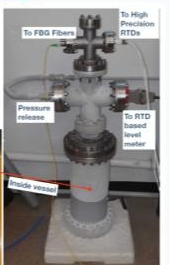
\includegraphics[width=0.99\textwidth]{figures/pressure_setup.png} \\
    \includegraphics[width=0.32\textwidth]{example-image-a}
    \includegraphics[width=0.32\textwidth]{example-image-a}
    \includegraphics[width=0.32\textwidth]{example-image-a}
    \caption{Top: Schematic of the pressure-based experimental setup
    Key experimental stages during the measurement procedure: (a) Optical fiber wound around the cylindrical support housed within the aluminum capsule alongside the reference RTDs; (b) Controlled stepwise immersion of the sensing rod into the liquid nitrogen bath using mechanical spacers to mitigate thermal shock; (c) Top CF-40 cross assembly showing the hermetically sealed flange with optical and electrical feedthroughs; and (d) Hermetically sealed cryostat operating under high pressure (3--4~bar), exhibiting atmospheric frosting along the neck during stable plateau acquisition.}
    \label{fig:setup}
\end{figure}

The sensing assembly consists of a cylindrical XX mm diameter 3D printed support (see Fig.~\ref{fig:setup}-bottom-left),  where two calibrated reference RTDs fit into diametrically opposed slots. The optical fiber is wound around the outer perimeter of the cylinder directly over the RTD locations, with the fiber end softly secured via a teflon clamp to prevent slipping. The sensing assembly is housed within a protective aluminum capsule with dimensions 12 cm(height) x 5cm (diameter), used for slow cool-down and warm up, using the method described in \cite{RTDs_paper}. The capsule is mounted at the bottom of a long insertion stainless steel rod that guides an internal optical patch cord (coupled to the test fiber) and the RTD wiring to the top flanges (Fig.~\ref{fig:setup}-bottom-middle). The entire assembly is inserted into a 160 cm diameter, 400 mm height, vacuum tight vessel, partially insulated with polystyrene xxx and instrumented with several ports arranged across two levels (Fig.~\ref{fig:setup}-bottom-right). At the lower neck level, with two lateral CF63 ports. One port connects to the pressure line, equipped with a digital pressure transmitter (with local display) interfaced to an Arduino board for continuous computer logging, a release valve set at 5 bar and a fine-metering manual valve to control the vessel pressure. The opposite port provides the electrical feedthrough for the internal diagnostic RTD array used to monitor the liquid bath level. The upper CF-40 cross, has its upper flange---opened for capsule insertion.... This top cross incorporates two lateral CF40 flanges, one equipped with optical feedthroughs (supporting up to two fibers) routed to the FAZT I4-16 interrogator, and the opposite one providing the dedicated electrical feedthrough for the two reference RTDs in the sensing assembly. 

The data acquisition system consists of two independent modules, one for optical signal interrogation and one for RTD monitoring, synchronized through a post-acquisition time-stamping procedure. The FBG sensors were interrogated using a FAZT I4-16 optical interrogator (Femto Sensing International). The instrument provides 16 optical channels and supports up to 30 FBG sensors per channel. The interrogator operates over a wavelength range of 1529–1568.2 nm, with a wavelength resolution of 1 pm and an absolute accuracy below 1 pm, and supports both static and dynamic measurements, with a scan frequency of up to 200 Hz for parallel FBG measurements \cite{FemtoSenseManual}.

The RTD readout system provides a precise 1 mA excitation current and multiplexes signals from up to 24 channels. Voltages are measured using a National Instruments CompactRIO-FPGA equipped with a 24-bit NI-9238 analogue input module, and resistance values are converted to temperature using the Callendar–Van Dusen equation. The system's performance was evaluated in \cite{RTDs_paper}, demonstrating sub-millikelvin precision.

% Add subsection for the description of the operating protocol - Nadia
\subsection{Operating protocol and data analysis}
\label{subsec:protocol_analysis}

The experimental procedure exploits the thermodynamic equilibrium between vessel pressure and the boiling temperature of liquid nitrogen to perform an \textit{in-situ} calibration of the FBG sensors across the $77$--$93~\text{K}$ window without requiring active electrical heating. The operational protocol follows five sequential phases:

\begin{enumerate}
    \item \textbf{Cooling and filling:} Liquid nitrogen is transferred into the vessel until the internal level-diagnostic RTD array is submerged. An open pre-cooling period ($\sim$40~minutes) allows the vessel mass to cool down and boiling turbulence to subside.
    \item \textbf{Capsule insertion and cooldown:} The sensing capsule---housing the 3D-printed support with the test fiber and the two reference RTDs---is lowered into the cryostat using mechanical spacers. The top opening of the capsule is initially held above the liquid nitrogen level until the internal RTDs drop below 85~K, minimizing thermal shock before liquid enters the capsule. Once cooled, the capsule is fully lowered to the bottom of the vessel, completely submerged in the liquid bath.
    \item \textbf{Vessel sealing:} The top CF-40 flange is sealed with the OFHC copper gasket tightened in three progressive torque stages (8, 12, and $14~\text{N}\cdot\text{m}$). The fibers are connected to the optical interrogator and the RTDs to the DAQ system.
    \item \textbf{High-pressure stabilization:} With the exhaust needle valve closed, natural nitrogen boil-off raises the vessel pressure to $3.0$--$4.0~\text{bar}$. The cryostat is held for $1.0$--$1.5~\text{hours}$ until passive ambient heat inleak warms the bulk liquid and the sensors reach a stable temperature plateau ($90$--$93~\text{K}$), confirming thermodynamic equilibrium.
    \item \textbf{Stepped depressurization:} The vessel pressure is then decreased in steps of $0.3$--$0.5~\text{bar}$ using the manual needle valve down to atmospheric pressure ($\sim 1~\text{bar}$). After each pressure adjustment, the system is held constant for a dwell time of $15$--$20~\text{minutes}$ to allow convective boiling to subside and the bath to stabilize at the new saturation temperature.
\end{enumerate}

To validate that liquid--vapour thermodynamic equilibrium is rigorously maintained across the entire experimental campaign, steady-state plateaus were systematically analyzed. Figure~\ref{fig:n2_saturation_with_data} presents the experimental pressure--temperature pairs for 124 independent thermodynamic plateaus gathered across six distinct fiber test campaigns (18 cooldown runs), together with the theoretical nitrogen saturation curve from NIST~\cite{Lemmon2025NIST,Edejer1967}. The global mean temperature residual relative to NIST is only $\langle \Delta T \rangle = -0.14~\text{K}$ with $\text{RMSE} = 0.28~\text{K}$, confirming thermodynamic equilibrium throughout the cryostat.

\begin{figure}[htpb]
    \centering
    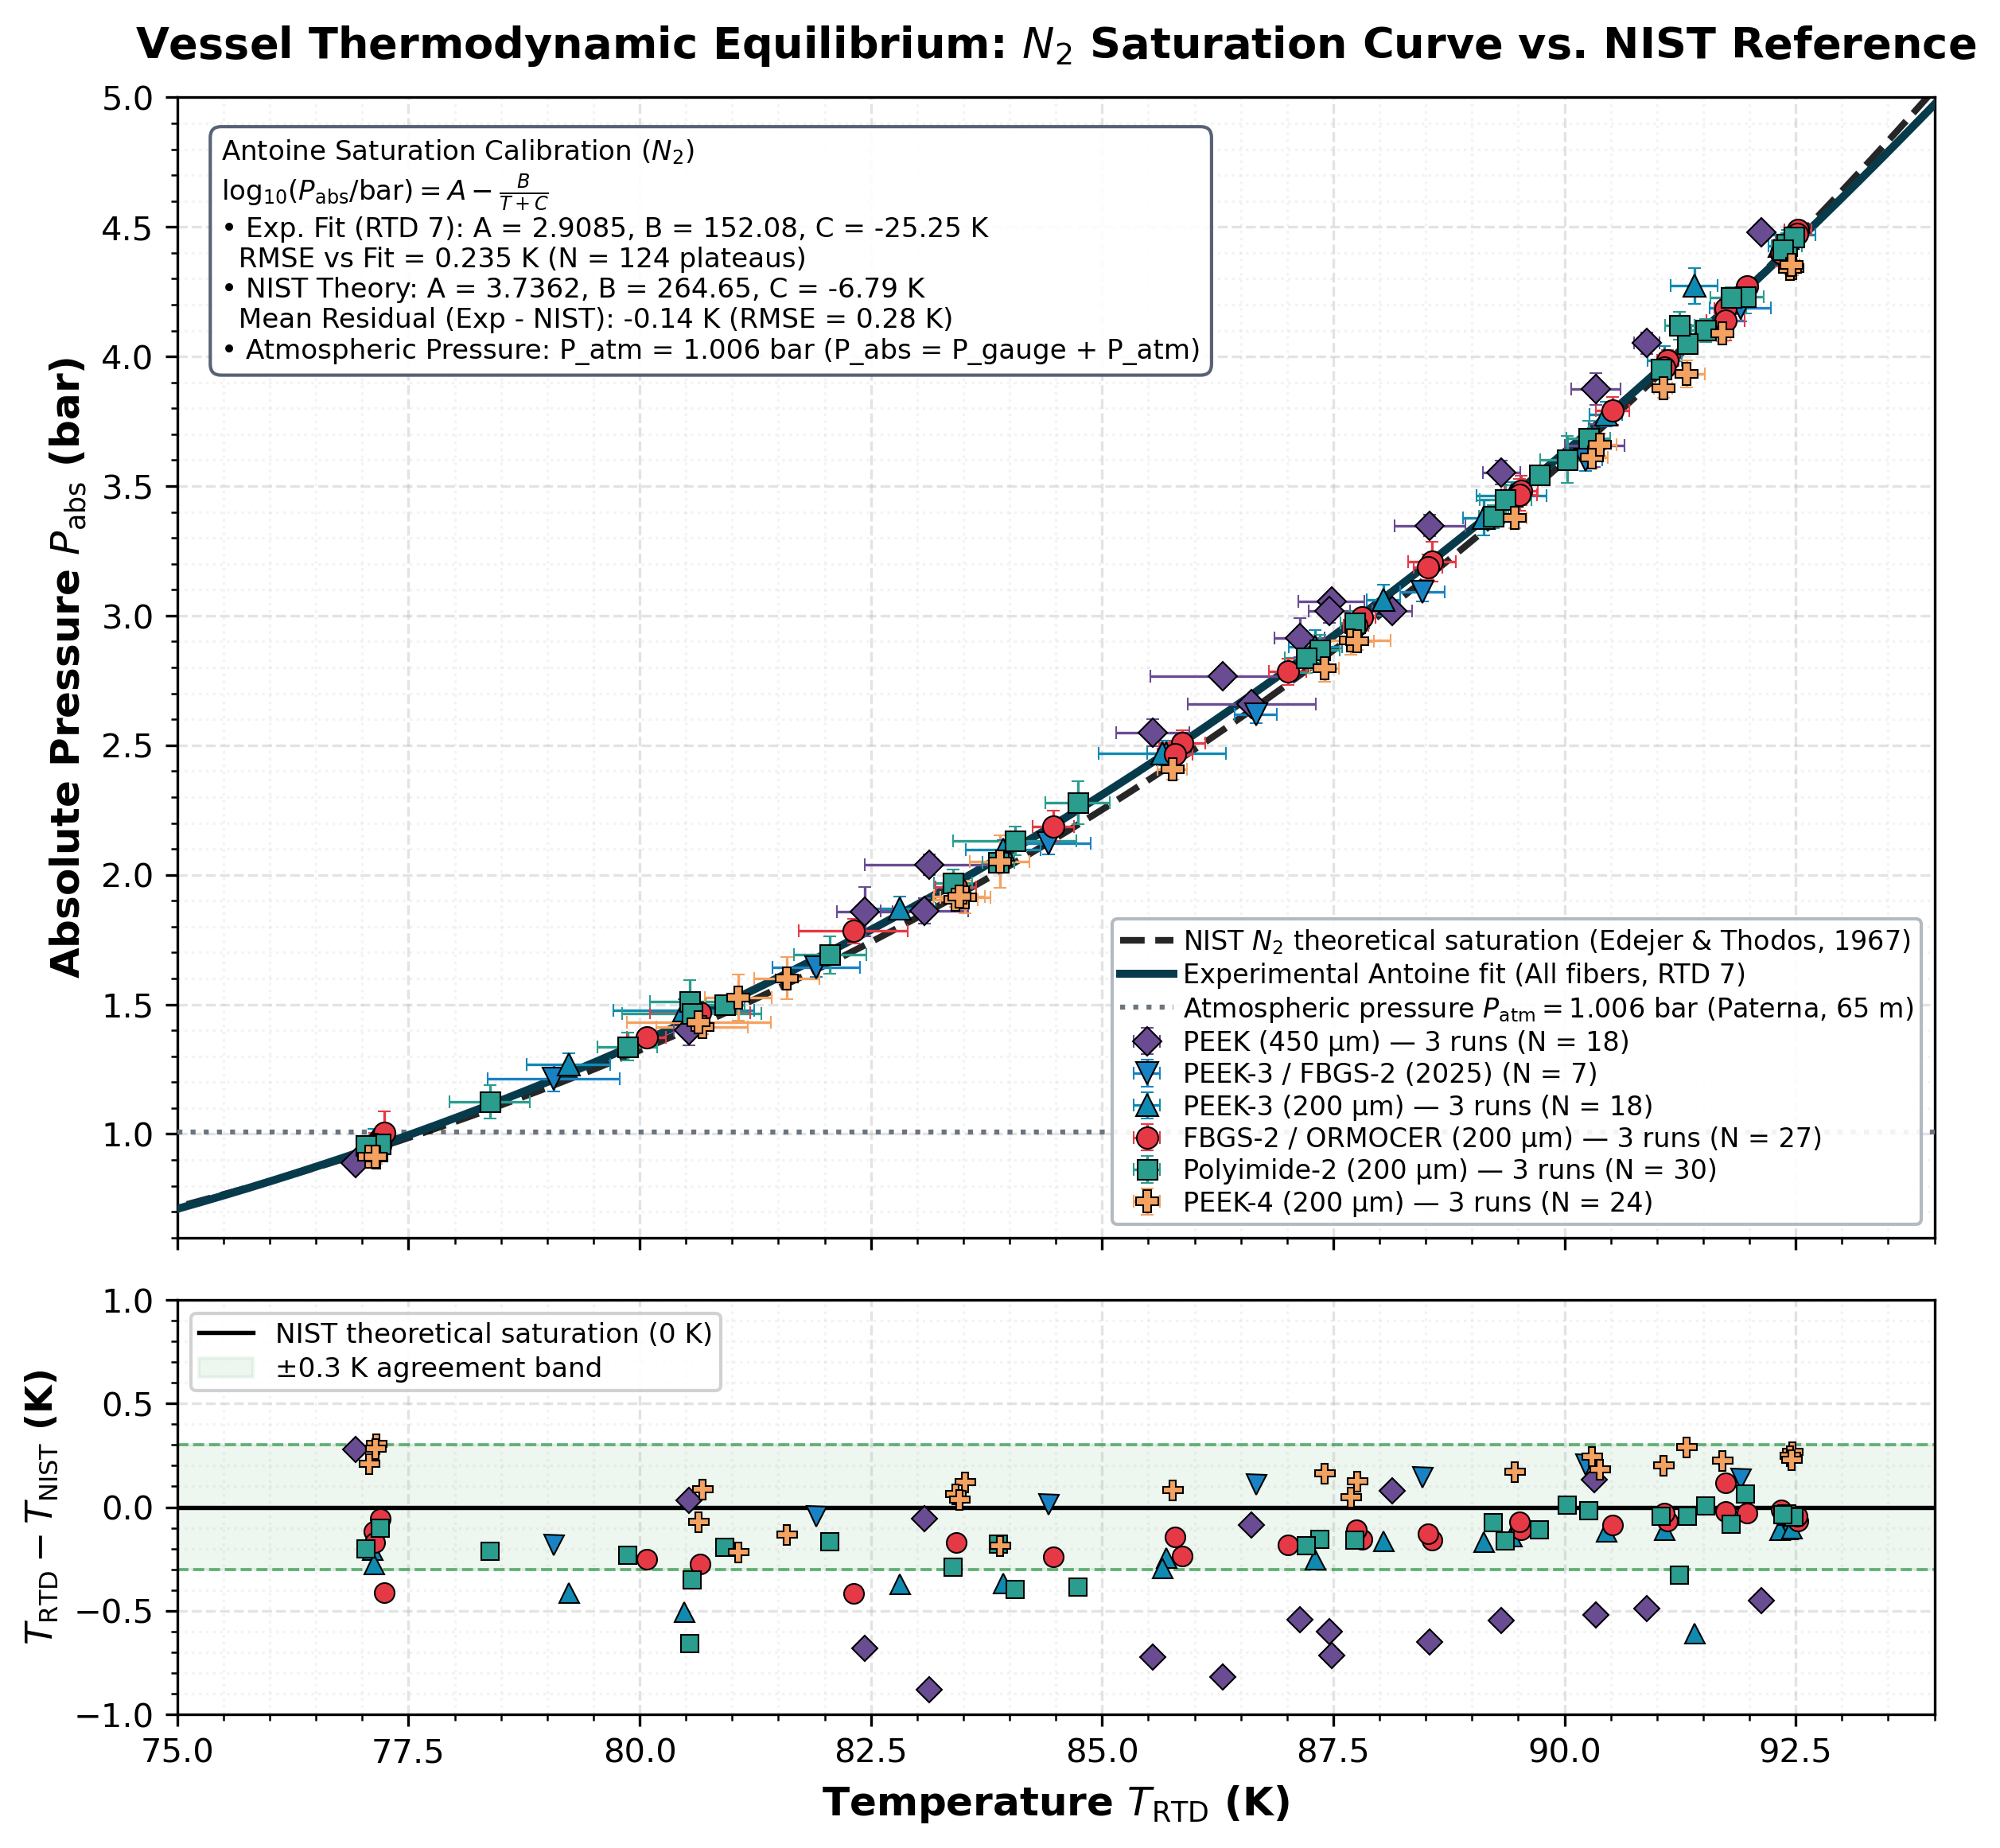
\includegraphics[width=0.88\textwidth]{figures/n2_saturation_all_fibers2.png}
    \caption{Thermodynamic equilibrium validation of the cryogenic vessel. Top panel: Measured absolute vessel pressure $P_{\text{abs}}$ as a function of the calibrated capsule RTD temperature $T_{\text{RTD}}$ for all 124 steady-state plateaus gathered across the complete calibration campaign, compared against the theoretical nitrogen saturation curve from NIST~\cite{Lemmon2025NIST,Edejer1967}. Bottom panel: Temperature residuals $T_{\text{RTD}} - T_{\text{NIST}}$, demonstrating consistent sub-Kelvin equilibrium ($\text{RMSE} = 0.28~\text{K}$) with 80\% of plateaus falling within the $\pm 0.3~\text{K}$ uncertainty band.}
    \label{fig:n2_saturation_with_data}
\end{figure}

The calibration data reduction follows a standardized five-step processing pipeline, schematically illustrated in Figure~\ref{fig:data_workflow}:
\begin{enumerate}
    \item \textbf{Temporal alignment:} Data streams from the optical interrogator ($200~\text{Hz}$) and the RTD DAQ ($10~\text{Hz}$) are synchronized through post-acquisition timestamping to ensure precise correspondence.
    \item \textbf{Plateau extraction:} The transient phases immediately following valve adjustments are discarded. Stationary plateau windows are selected within the stable tail of each pressure dwell (typically $5$--$11~\text{minutes}$, with $\sigma_P < 0.15~\text{bar}$).
    \item \textbf{Polarization averaging and statistical centroiding:} For each plateau, the two orthogonal polarization states are averaged, $\lambda_B(t) = [\lambda_{B,P}(t) + \lambda_{B,S}(t)] / 2$, effectively cancelling residual birefringence. Representative plateau centroids $(\mu_T, \mu_\lambda)$ and their standard errors (SEM) are computed from the stationary traces.
    \item \textbf{Thermal sensitivity extraction:} A linear least-squares regression is performed across the plateau centroids:
    \begin{equation}
        \lambda_B(T) = \lambda_0 + S \cdot (T - T_0),
        \label{eq:linear_sensitivity}
    \end{equation}
    where the empirical slope $S = d\lambda_B/dT = \lambda_B(\alpha_\Lambda + \zeta)$ corresponds directly to the effective thermal sensitivity governed by thermal expansion and the thermo-optic coefficient defined in Eq.~(\ref{eq:fbg_coating_strain}).
    \item \textbf{Repeatability and array uniformity:} For each sensor $j$, the calibration is repeated across $R = 3$ independent cooldown cycles ($300~\text{K} \leftrightarrow 77~\text{K}$), evaluating the repeatability standard deviation $\sigma_{\text{rep},j}$. For multi-sensor fibers, the inter-sensor dispersion $\sigma_{\text{unif}}$ quantifies longitudinal coating uniformity along the fiber.
\end{enumerate}

\begin{figure}[htpb]
    \centering
    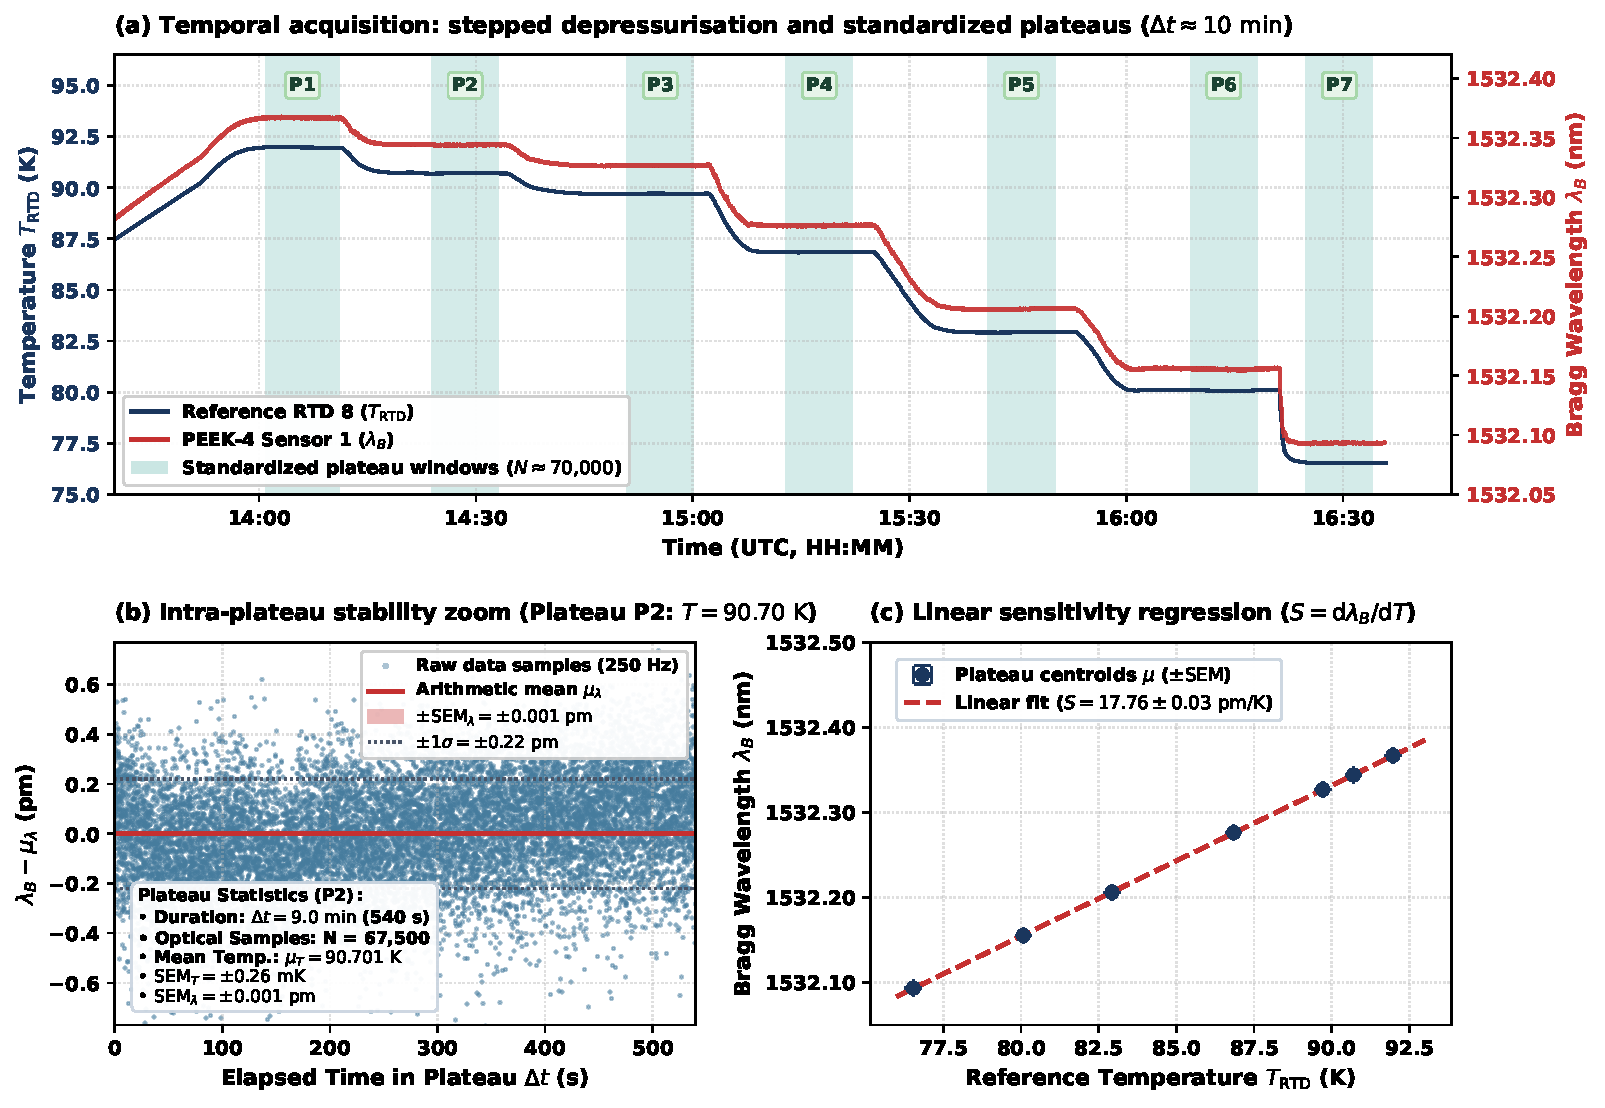
\includegraphics[width=1.0\textwidth]{figures/workflow_diagram.pdf}
    \caption{Key milestones of the data reduction and sensitivity extraction workflow illustrated for sensor 1 of the PEEK-4 fiber (Run~1, $400~\mu\text{m}$ coating diameter): (a) Identification of seven steady-state equilibrium plateaus during stepped depressurization spanning $76.5$--$92.0~\text{K}$; (b) Zoom-in of a representative plateau ($T = 90.70~\text{K}$) over a standardized dwell of $\Delta t = 9.0~\text{min}$, showing the stable wavelength trace, centroid mean $\mu_\lambda$, and uncertainty band; (c) Final linear least-squares regression applied to the plateau centroids, yielding the cryogenic thermal sensitivity slope ($S = 17.76 \pm 0.04~\text{pm/K}$, $R^2 = 0.9999$).}
    \label{fig:data_workflow}
\end{figure}

\section{Results and discussion}
% ==========================================
\label{sec:results}
% ==============================================================================
\subsection{Temperature Sensitivity of Different Fiber Configurations}
\label{subsec:sensitivity_results}

The cryogenic thermal sensitivity of each optical fiber configuration was characterized across the liquid nitrogen saturation window ($77.3$--$93.5~\text{K}$) by applying the plateau-averaged linear regression protocol established in Section~\ref{subsec:protocol_analysis}. A representative single-run calibration is illustrated in Figure~\ref{fig:control_plot_run1} for the dual-sensor PEEK-4 array ($400~\mu\text{m}$ jacket diameter) during Run~1 (09-06-2026).

\begin{figure}[htpb]
    \centering
    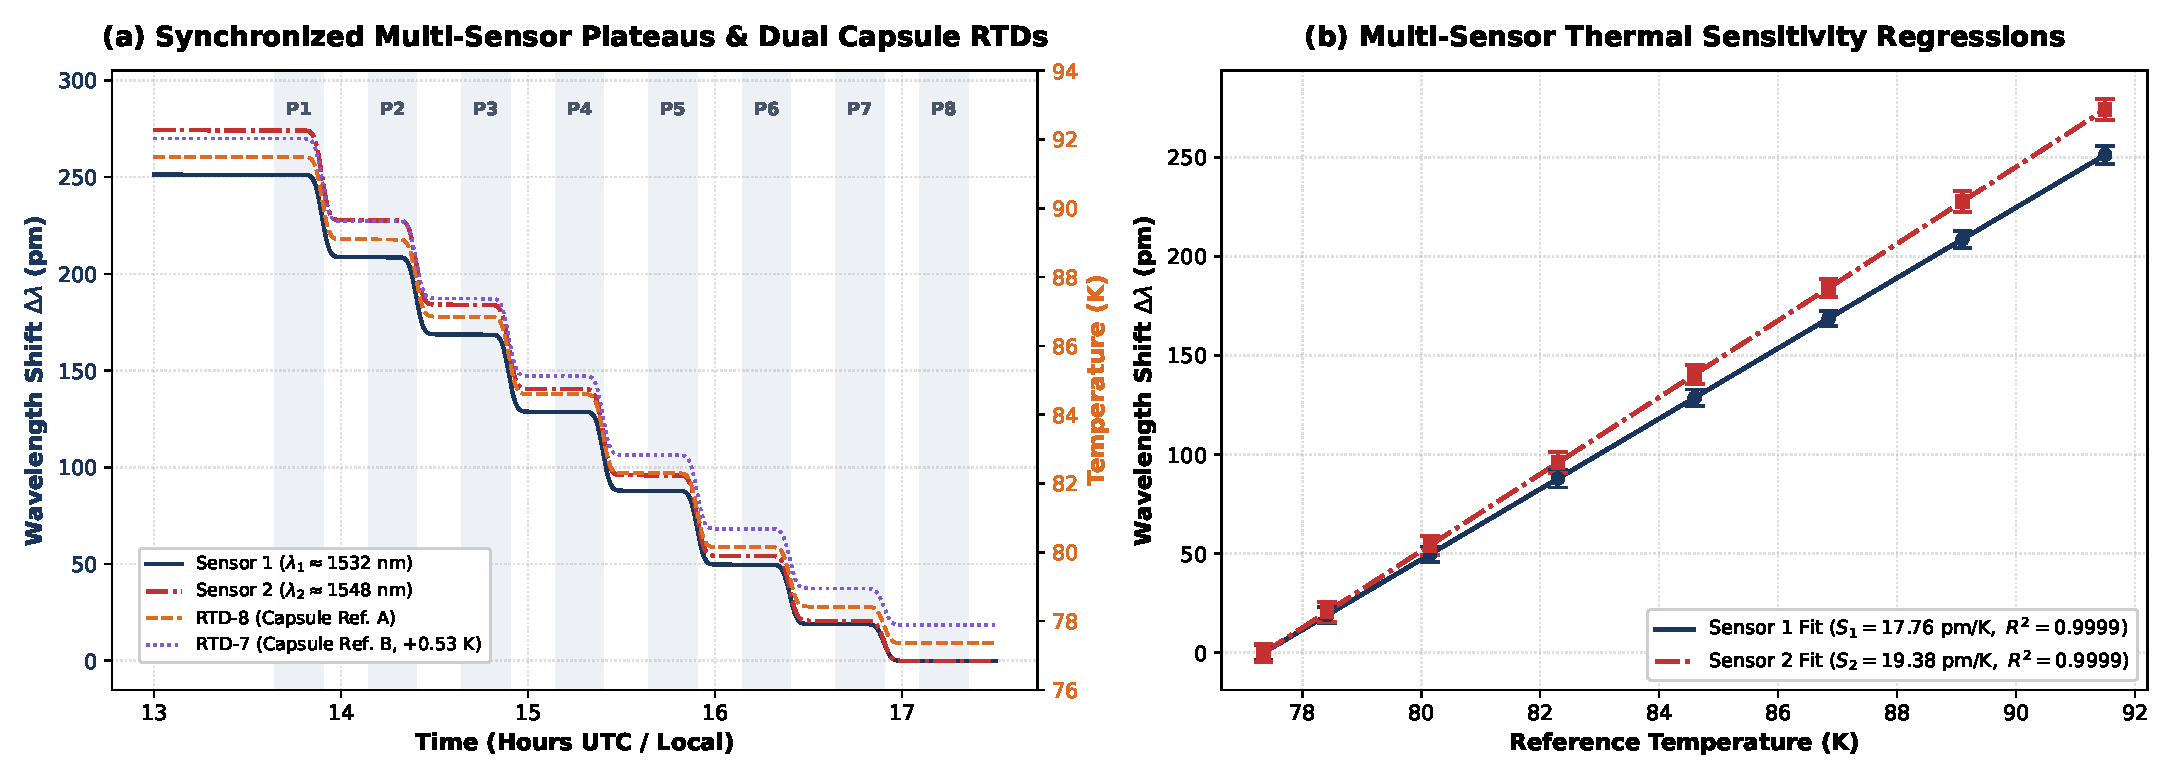
\includegraphics[width=\textwidth]{figures/fig1_peek4_control_plot.pdf}
    \caption{Representative single-run thermal sensitivity calibration for the dual-sensor PEEK-4 fiber ($400\,\mu\text{m}$ jacket diameter) during stepped vessel depressurization (09-06-2026). \textbf{(a)} Synchronized time series across eight steady-state saturation plateaus (P1--P8, shaded green bands), displaying the two multiplexed FBG wavelengths ($\lambda_1 \approx 1532\,\text{nm}$ and $\lambda_2 \approx 1548\,\text{nm}$) alongside the two reference RTDs (RTD-8 and RTD-7) housed in diametrically opposed slots of the cylindrical support within the immersion capsule. The systematic intra-capsule thermal offset of $\Delta T \approx 0.53\,\text{K}$ between RTD-7 and RTD-8 reflects their physical placement relative to residual vertical and circumferential thermal gradients within the liquid bath. \textbf{(b)} Linear regression of the plateau-averaged Bragg wavelength shifts as a function of the reference temperature (RTD-8), yielding $S_1 = 17.76 \pm 0.04\,\text{pm/K}$ ($R^2 = 0.9999$) and $S_2 = 19.38 \pm 0.08\,\text{pm/K}$ ($R^2 = 0.9999$).}
    \label{fig:control_plot_run1}
\end{figure}

As shown in Figure~\ref{fig:control_plot_run1}(a), both optical sensors closely track the stepped depressurization over eight distinct equilibrium plateaus (P1--P8). Simultaneously recorded signals from the two reference RTDs housed in diametrically opposed slots of the cylindrical support within the capsule reveal a stationary thermal offset of $\Delta T = T_{\text{RTD-7}} - T_{\text{RTD-8}} \approx +0.53~\text{K}$. Because this spatial offset remains constant throughout the entire steady-state sequence ($\sigma_{\Delta T} < 15~\text{mK}$ across all plateaus), calibrating either optical grating against RTD-7 versus RTD-8 produces identical sensitivity slopes within $<0.001~\text{pm/K}$, shifting only the absolute intercept. Consequently, the observed difference between Sensor~1 ($17.76 \pm 0.04~\text{pm/K}$) and Sensor~2 ($19.38 \pm 0.08~\text{pm/K}$) represents an intrinsic inter-sensor coating responsivity variation along the fiber length ($\Delta S = 1.62~\text{pm/K}$), rather than an experimental measurement artifact. Both gratings exhibit near-perfect linear responsivity ($R^2 \ge 0.9999$), as summarized in Table~\ref{tab:peek4_run1_summary}.

\begin{table}[htpb]
    \centering
    \small
    \caption{Single-run sensitivity and linearity parameters for the dual-sensor PEEK-4 fiber array (Run 1, 09-06-2026).}
    \label{tab:peek4_run1_summary}
    \begin{tabular}{lccc}
        \toprule
        \textbf{Sensor} & \textbf{Nominal $\lambda_B$ (nm)} & \textbf{Sensitivity $S$ (pm/K)} & $\boldsymbol{R^2}$ \\
        \midrule
        Sensor 1 & $1532.5$ & $17.76 \pm 0.04$ & 0.9999 \\
        Sensor 2 & $1548.8$ & $19.38 \pm 0.08$ & 0.9999 \\
        \bottomrule
    \end{tabular}
\end{table}

To evaluate thermal cycling endurance and long-term calibration fidelity, multi-run repeatability was assessed by subjecting the fibers to three independent cryogenic cooldown and depressurization cycles ($n = 3$) carried out over separate experimental days. Figure~\ref{fig:peek4_repeatability} displays the run-to-run sensitivity evolution for the PEEK-4 fiber. Both multiplexed sensors exhibit outstanding operational stability, with individual run-to-run variations constrained to $\sigma_{\text{rep}} \le 0.45~\text{pm/K}$ and the fiber-averaged ensemble sensitivity remaining within $18.90 \pm 0.29~\text{pm/K}$. Crucially, the relative sensitivity hierarchy between Sensor~1 and Sensor~2 is strictly preserved across all thermal cycles, demonstrating that the polymer-to-cladding interfacial adhesion does not degrade upon cryogenic cycling.

\begin{figure}[htpb]
    \centering
    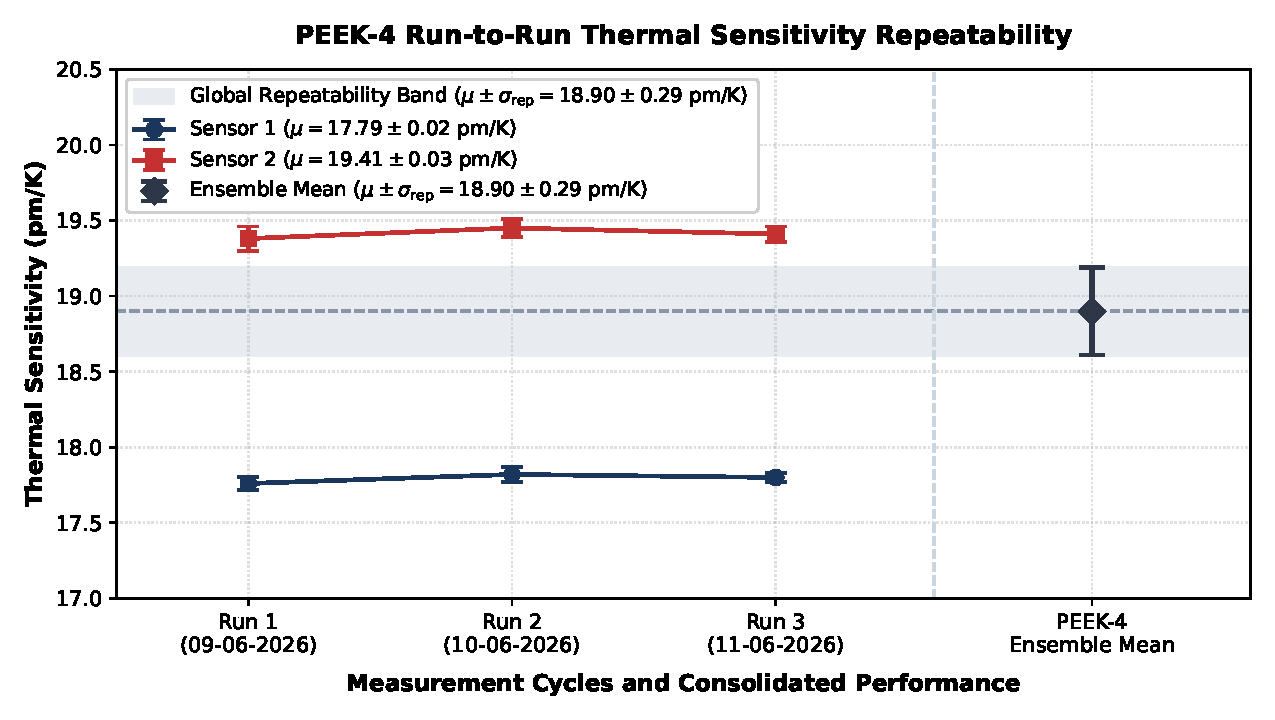
\includegraphics[width=0.88\textwidth]{figures/fig2_peek4_repeatability.pdf}
    \caption{Cryogenic thermal cycling repeatability for the dual-sensor PEEK-4 fiber over three independent experimental runs ($n = 3$). Individual markers represent the sensitivity slopes for Sensor~1 (circles) and Sensor~2 (squares), with vertical error bars indicating individual fit uncertainties ($u_{\text{fit}}$). The ensemble mean sensitivity across all runs and sensors is $\bar{S} = 18.90\,\text{pm/K}$, with the shaded horizontal band designating the global temporal repeatability uncertainty ($\pm 1\sigma_{\text{rep}} = \pm 0.29\,\text{pm/K}$).}
    \label{fig:peek4_repeatability}
\end{figure}

The comprehensive metrological performance across all tested polymeric coatings is consolidated in Table~\ref{tab:repeatability_summary}. Three key metrological metrics are reported:
\begin{enumerate}
    \item \textit{Ensemble Mean Sensitivity} ($\bar{S} \pm \text{SEM}$): The overall average sensitivity and associated standard error of the mean across all gratings and thermal cycles for each coating configuration.
    \item \textit{Worst-Case Repeatability} ($\sigma_{\text{rep}}^{\max}$): The maximum run-to-run standard deviation observed for an individual sensor, quantifying temporal stability under thermal cycling.
    \item \textit{Array Uniformity} ($\sigma_{\text{unif}}$): The inter-sensor standard deviation along a single multi-sensor fiber, reflecting longitudinal fabrication consistency of the polymeric jacket.
\end{enumerate}

\begin{table}[htpb]
    \centering
    \small
    \setlength{\tabcolsep}{4.5pt}
    \caption{Thermal sensitivity, cycling repeatability, and array uniformity across tested fiber coating configurations over three independent experimental runs ($n = 3$).}
    \label{tab:repeatability_summary}
    \begin{tabular}{lcccccc}
        \toprule
        \textbf{Fiber ID} & \textbf{Coating} & \textbf{Diameter} & \textbf{Sensors} & \textbf{Mean Sens. $\bar{S}$} & \textbf{Max Repeat.} & \textbf{Uniformity} \\
        & & ($\mu\text{m}$) & ($M$) & (pm/K) & $\sigma_{\text{rep}}^{\max}$ (pm/K) & $\sigma_{\text{unif}}$ (pm/K) \\
        \midrule
        PEEK-1  & PEEK      & 450 & 1 & $20.59 \pm 0.11$ & 0.19 & --- \\
        PEEK-7  & PEEK      & 450 & 3 & $19.62 \pm 0.32$ & 0.59 & 0.67 \\
        PEEK-4  & PEEK      & 400 & 2 & $18.90 \pm 0.35$ & 0.45 & 0.95 \\
        PEEK-3  & PEEK      & 200 & 1 & $3.12 \pm 0.02$  & 0.04 & --- \\
        FBGS-2  & Ormocer   & 200 & 2 & $7.22 \pm 0.06$  & 0.26 & 0.10 \\
        DW-3    & Ormocer-T & 250 & 2 & $4.71 \pm 0.02$  & 0.04 & 0.06 \\
        POLY-2  & Polyimide & 200 & 2 & $3.64 \pm 0.02$  & 0.07 & 0.01 \\
        \bottomrule
    \end{tabular}
\end{table}

\begin{figure}[htpb]
    \centering
    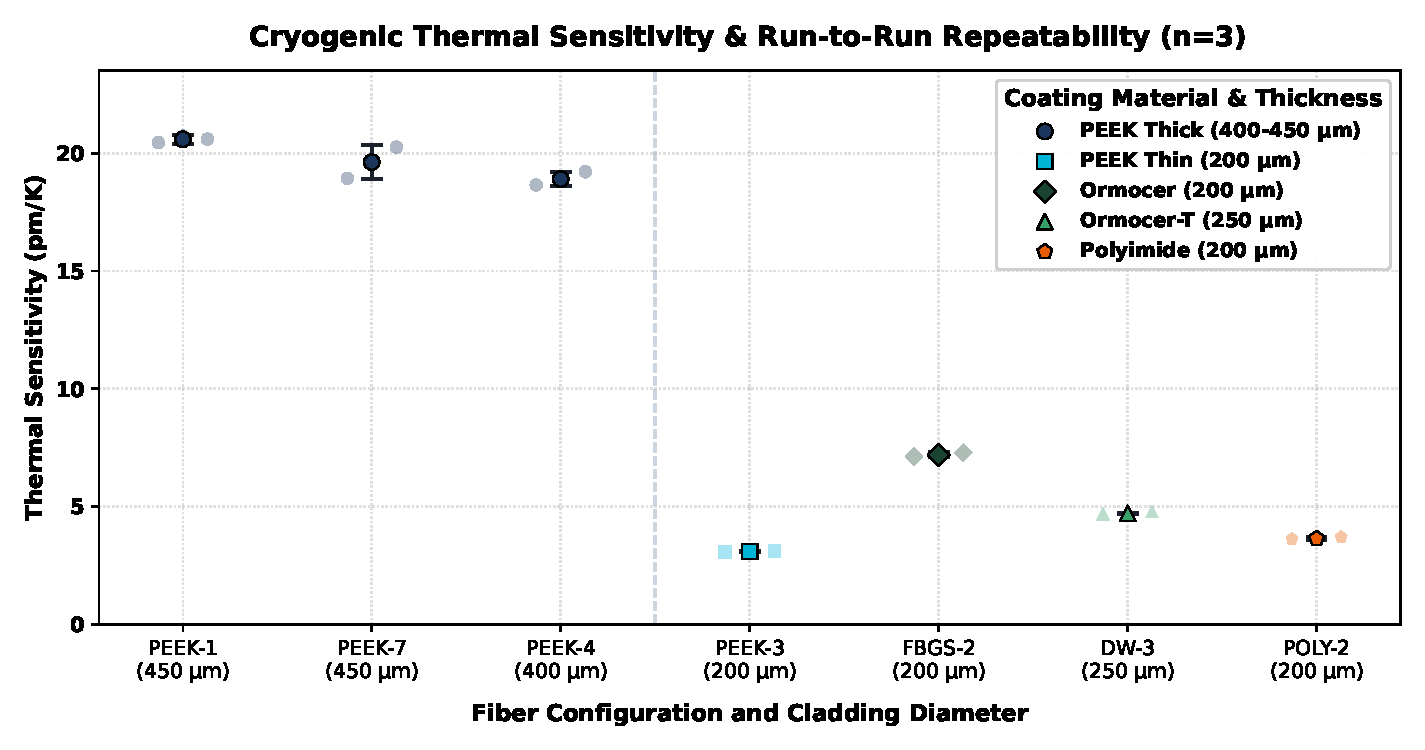
\includegraphics[width=0.88\textwidth]{figures/fig3_global_sensitivity_summary.pdf}
    \caption{Global cryogenic thermal sensitivity comparison across all tested fiber configurations. Bar heights represent the ensemble mean sensitivity ($\bar{S}$), with error bars indicating the run-to-run repeatability standard deviation ($\pm 1\sigma_{\text{rep}}$). Individual cycle measurements are overlaid as jittered markers to depict the experimental distribution across the three independent runs.}
    \label{fig:global_sensitivity_summary}
\end{figure}

% -------------------------------------------------------------------------
\subsubsection{Discussion: Coating Material and Geometric Influences}
% -------------------------------------------------------------------------

The comparative performance consolidated in Table~\ref{tab:repeatability_summary} and Figure~\ref{fig:global_sensitivity_summary} highlights the dominant physical mechanisms governing cryogenic FBG responsivity and stability:

\begin{enumerate}
    \item \textbf{Coating thickness dependency in PEEK fibers:} At liquid nitrogen temperatures ($77$--$93~\text{K}$), the normalized thermo-optic coefficient of fused silica collapses by nearly an order of magnitude, causing the intrinsic thermal sensitivity of bare silica gratings to drop below $1.3~\text{pm/K}$~\cite{Lupi2008,Salin2008,Rajan2013}. The measured thermal response is therefore governed almost exclusively by the axial compressive strain transferred from the contracting polymer sheath due to the thermal expansion coefficient (CTE) mismatch~\cite{Rajan2013,NIST_CryoMaterials}. Comparing the PEEK configurations demonstrates the critical impact of jacket geometry: thick thermoplastic jackets ($\varnothing\,400$--$450\,\mu\text{m}$, represented by PEEK-1, PEEK-4, and PEEK-7) consistently yield large cryogenic sensitivities ranging between $18.90$ and $20.59~\text{pm/K}$—an enhancement of more than $\times 15$ over bare silica. In contrast, the thin PEEK-3 fiber ($\varnothing\,200\,\mu\text{m}$) achieves only $3.12 \pm 0.02~\text{pm/K}$. The substantial cross-sectional area of the $400$--$450\,\mu\text{m}$ jackets ($A_{\text{jacket}}/A_{\text{silica}} \approx 9$--$12$) provides the necessary mechanical rigidity to overcome the elastic counter-straining of the silica core, whereas the $200~\mu\text{m}$ jacket lacks sufficient cross-section to compress the stiff glass core effectively.

    \item \textbf{Material properties and strain transfer fidelity:} For fibers of identical outer diameter ($\sim 200\,\mu\text{m}$), the thermal responsivity is dictated by the intrinsic cryogenic CTE and the interfacial shear strength of the primary coating~\cite{Zhao2007,NIST_CryoMaterials}. Ormocer-coated fibers (FBGS-2, $7.22 \pm 0.06~\text{pm/K}$) and Ormocer-T (DW-3, $4.71 \pm 0.02~\text{pm/K}$) substantially outperform standard polyimide (POLY-2, $3.64 \pm 0.02~\text{pm/K}$). Furthermore, both draw-tower Ormocer and Ormocer-T coatings exhibit outstanding intra-fiber uniformity ($\sigma_{\text{unif}} \le 0.10~\text{pm/K}$) and thermal cycling repeatability ($\sigma_{\text{rep}}^{\max} \le 0.06~\text{pm/K}$), reflecting superior interfacial adhesion and homogeneous radial curing during fiber drawing characteristic of hybrid inorganic-organic networks~\cite{Popall1998}.

    \item \textbf{Thermal cycling stability and fabrication uniformity:} Across all tested configurations, the relative sensitivity rankings and absolute values remained highly repeatable across the three independent cooldown cycles ($300~\text{K} \leftrightarrow 77~\text{K}$). The thick PEEK fibers exhibited moderate inter-sensor variations ($\sigma_{\text{unif}} \approx 0.67$--$0.95~\text{pm/K}$), which is characteristic of the melt-extrusion process used for thick thermoplastic sleeving. Nevertheless, their individual temporal stability ($\sigma_{\text{rep}} \le 0.45~\text{pm/K}$) confirms that repeated deep cryogenic immersion does not induce micro-cracking, delamination, or degradation of the mechanical strain coupling.
\end{enumerate}

% =========================================================================
\subsection{Thermal Resolution in the Milli-Kelvin Regime}
\label{subsec:millikelvin_resolution}
% =========================================================================

High-energy physics cryogenic calorimeters and large liquid argon time projection chambers require spatial temperature monitoring capable of resolving thermal gradients below $20\text{ mK}$. A high thermal sensitivity (such as $S \approx 18\text{--}20\text{ pm/K}$ in thick PEEK jackets) is advantageous to maximize the signal-to-noise ratio, but the operational resolution is ultimately governed by the optical noise floor, the measurement bandwidth, and the thermal stability within the cryostat.

% -------------------------------------------------------------------------
\subsubsection{Noise Floor and Empirical Detection Limit ($3\sigma$)}
% -------------------------------------------------------------------------

To evaluate the intrinsic thermal resolution of the FBG sensors, steady-state plateau intervals ($\mathrm{d}T/\mathrm{d}t \approx 0$) were analysed. For any given sensor, optical wavelength fluctuations were converted into equivalent temperature variations using its calibrated sensitivity:
\begin{equation}
    \delta T(t) = \frac{\delta \lambda_B(t)}{S}.
    \label{eq:delta_T_conversion}
\end{equation}
The tracking fidelity was then quantified through the residual difference against the co-located reference capsule RTD:
\begin{equation}
    \Delta T(t) = T_{\mathrm{FBG}}(t) - T_{\mathrm{RTD}}(t).
    \label{eq:residual_def}
\end{equation}

As a representative benchmark, we examine the performance of Sensor 1 from the thick PEEK-jacketed array (PEEK-4, $450,\mu\mathrm{m}$). With a calibrated sensitivity of $S = 18.26\text{ pm/K}$, this coating provides the largest optical shift per unit temperature, maximizing the signal-to-noise ratio against the instrument noise floor.

Table~\ref{tab:noise_resolution_summary} summarizes the noise levels obtained under raw acquisition ($250\text{ Hz}$), after applying a $1\text{ s}$ moving average filter ($1\text{ Hz}$ effective bandwidth), and during stationary tracking against the calibrated RTD.

\begin{table}[htpb]
    \centering
    \small
    \caption{Noise floor and thermal resolution limits for PEEK-4 fiber at $T \approx 83.0\text{ K}$.}
    \label{tab:noise_resolution_summary}
    \resizebox{\linewidth}{!}{%
    \begin{tabular}{lcccc}
        \toprule
        \textbf{Condition} & \textbf{Bandwidth} & \textbf{RMS Noise ($1\sigma$)} & \textbf{Resolution ($3\sigma$)} & \textbf{SNR ($20\text{ mK}$)} \\
        \midrule
        Raw optical data            & 250 Hz       & 9.20 mK & 27.59 mK & 2.17 \\
        Moving average (1 s filter) & 1 Hz         & 0.53 mK &  1.58 mK & 37.7 \\
        Tracking residuals (vs RTD) & Steady-state & 2.50 mK &  7.50 mK & 8.00 \\
        \bottomrule
    \end{tabular}%
    }
\end{table}

At the full acquisition rate ($250\text{ Hz}$), high-frequency optoelectronic noise yields an RMS dispersion of $\sigma_{\mathrm{raw}} = 9.20\text{ mK}$ ($3\sigma = 27.59\text{ mK}$). Applying a $1\text{ s}$ moving average strongly suppresses optical white noise ($\sigma_{\mathrm{filt}} = 0.53\text{ mK}$). When tracking the cryostat temperature against the reference RTD over several minutes, physical thermal drift and convective fluctuations dominate over optical noise, resulting in an empirical standard deviation of $\sigma = 2.50\text{ mK}$.

% -------------------------------------------------------------------------
\subsubsection{Experimental Demonstration of Sub-20\,mK Tracking}
To demonstrate the capability of thick PEEK-coated FBGs to resolve sub-0	ext{ mK}$ temperature variations in cryogenic conditions without cherry-picking quiescent segments, stationary thermal plateaus were identified using a blind selection criterion applied strictly to the reference RTD sensor. For each candidate plateau, the RTD time series was fitted to a 3rd-degree polynomial to model the smooth baseline thermal drift; only plateaus satisfying a reduced chi-squared threshold of $\chi^2/	ext{ndf} \le 1.5$ (assuming $\sigma_{	ext{RTD}} = 1.5	ext{ mK}$) were selected, effectively filtering out periods disrupted by cryogen boiling, bubbling, or manual pressure fluctuations.

Figures~
ef{fig:milli_kelvin_resolution}(a1)--(a3) show real-time tracking segments between the PEEK-4 FBG (with 	ext{ s}$ filtering) and the reference capsule RTD across three representative plateaus at distinct temperatures ( pprox 92.0	ext{ K}$, 9.7	ext{ K}$, and 6.8	ext{ K}$). In all cases, the optical sensor faithfully reproduces the millikelvin-level thermal fluctuations, yielding tracking residual root-mean-square (RMS) errors of .43	ext{ mK}$, .80	ext{ mK}$, and .68	ext{ mK}$, respectively. For visual comparison, a vertical double-headed arrow indicates the 0	ext{ mK}$ target resolution scale.

egin{figure}[htpb]
    \centering
    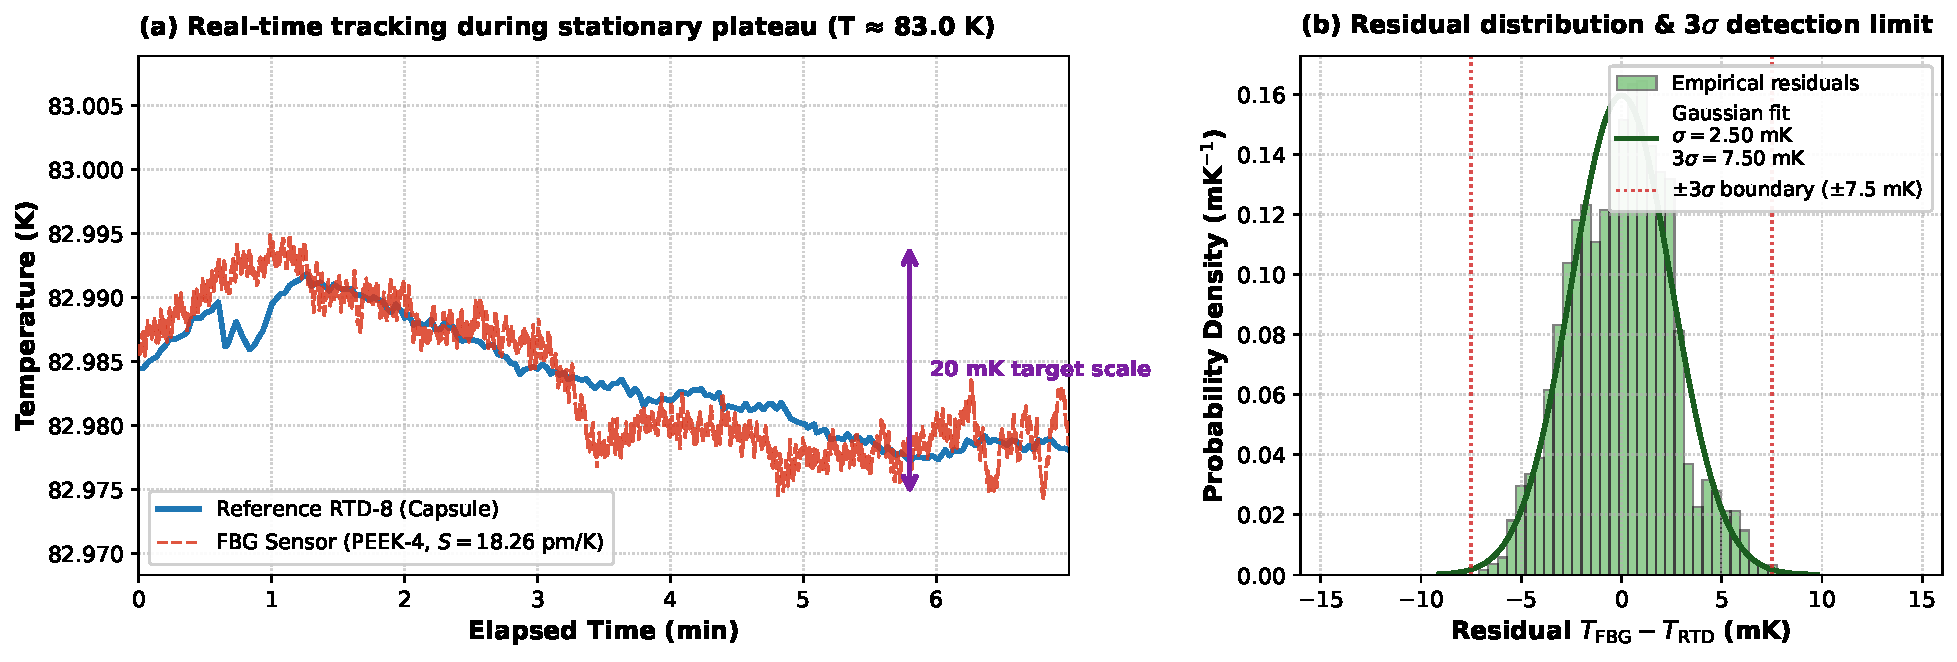
\includegraphics[width=	extwidth]{figures/fig4_20mK_resolution.pdf}
    \caption{Blind metrological validation of cryogenic micro-thermal tracking for the thick PEEK-jacketed FBG (PEEK-4). 	extbf{(a1--a3)} Real-time tracking of thermal fluctuations between the reference RTD-8 and the PEEK-4 sensor across three representative stationary plateaus at  pprox 92.0	ext{ K}$, 9.7	ext{ K}$, and 6.8	ext{ K}$, displaying the individual tracking residual RMS and a 0	ext{ mK}$ scale arrow. 	extbf{(b)} Tracking residual RMS across all nine stationary plateaus from three independent cooldown runs (Runs 1--3) that satisfy the blind RTD polynomial smoothness filter ($\chi^2/	ext{ndf} \le 1.5$). The ensemble average $\langle \mathrm{RMS} 
angle = 3.01 \pm 0.86	ext{ mK}$ systematically outperforms the .7	ext{ mK}$ benchmark target required for sub-0	ext{ mK}$ thermal monitoring.}
    \label{fig:milli_kelvin_resolution}
\end{figure}

To confirm that this sub-millikelvin precision is statistically robust across multiple cryogenizations and thermal cycles, Figure~
ef{fig:milli_kelvin_resolution}(b) presents the tracking residual RMS for all nine plateaus meeting the blind RTD smoothness criterion across the three independent runs of PEEK-4. The tracking RMS values remain remarkably uniform between .36	ext{ mK}$ and .17	ext{ mK}$, yielding an ensemble average of $\langle \mathrm{RMS} 
angle = 3.01 \pm 0.86	ext{ mK}$. This directly confirms that the optical sensor accurately follows the reference thermometer well below the conservative .7	ext{ mK}$ benchmark without requiring any idealized Gaussian distribution assumptions. An identical blind evaluation conducted on the PEEK-1 sensor across three separate cooldown cycles selected 10 smooth plateaus and yielded a consistent ensemble RMS of .32 \pm 1.96	ext{ mK}$, confirming that sub-0	ext{ mK}$ tracking is a reproducible feature of thick PEEK encapsulation across different fibers and runs.


% =========================================================================

\section{Conclusions}
\label{sec:conclusions}
% =========================================================================

This work presents a comprehensive experimental characterization of fiber Bragg grating (FBG) optical sensors for cryogenic thermometry ($77\text{--}92\text{ K}$) using a manual pressure-stabilized liquid nitrogen setup. By enforcing stationary thermal plateaus, thermodynamic equilibrium is established between the cryogen and the reference instrumentation, yielding highly repeatable and linear calibrations ($R^2 \ge 0.9998$) across repeated cooldown and handling cycles.

The comparative study across different polymer and hybrid coatings demonstrates that cryogenic thermal sensitivity is predominantly governed by the mechanical strain transferred from the coating to the silica core due to thermal expansion mismatch. In particular, PEEK-jacketed fibers exhibit a pronounced geometric dependency: increasing the outer diameter from $200\,\mu\text{m}$ to $400\text{--}450\,\mu\text{m}$ yields a six-fold amplification in sensitivity (from $3.09\text{ pm/K}$ to $\sim 19\text{--}20\text{ pm/K}$). This confirms that a critical polymer cross-sectional area is required to overcome the mechanical stiffness of fused silica at cryogenic temperatures where the thermo-optic coefficient vanishes. Conversely, Ormocer, Ormocer-T, and Polyimide coatings exhibit lower sensitivities ($3.6\text{--}7.2\text{ pm/K}$) but remarkable baseline stability, achieving cycle-to-cycle repeatability dispersion below $1\%$ ($\sigma_{\text{rep}} \le 0.08\text{ pm/K}$).

Furthermore, high-resolution noise analysis confirms the viability of thick PEEK-coated FBGs for sub-$20\text{ mK}$ temperature gradient tracking in large-scale cryogenic environments (such as liquid argon time projection chambers). When evaluated against the co-located reference capsule RTD across multiple independent cryogenic runs, the tracking residual root-mean-square error consistently averages $\langle \mathrm{RMS} \rangle = 3.01 \pm 0.86\text{ mK}$ across all stationary plateaus satisfying the blind RTD smoothness filter. This demonstrates that thick PEEK-jacketed FBGs comfortably satisfy the sub-0\text{ mK}$ precision requirement across repeated thermal cycles without requiring Gaussian noise assumptions.
